\documentclass[tikz,border=5pt]{standalone}
\usepackage[T1]{fontenc}
\usepackage{lmodern}
\usepackage{xcolor}
\usetikzlibrary{arrows.meta,calc}
\definecolor{ink}{HTML}{202020}
\definecolor{muted}{HTML}{565656}
\definecolor{rulegray}{HTML}{9A9A9A}
\definecolor{signal}{HTML}{3C607C}
\definecolor{wash}{HTML}{F4F4F4}
\definecolor{timing}{HTML}{685978}
\definecolor{delivery}{HTML}{8A6849}
\definecolor{participant}{HTML}{4F7563}
\newcommand{\labeltext}[1]{{\fontsize{7}{8.3}\selectfont #1}}
\begin{document}
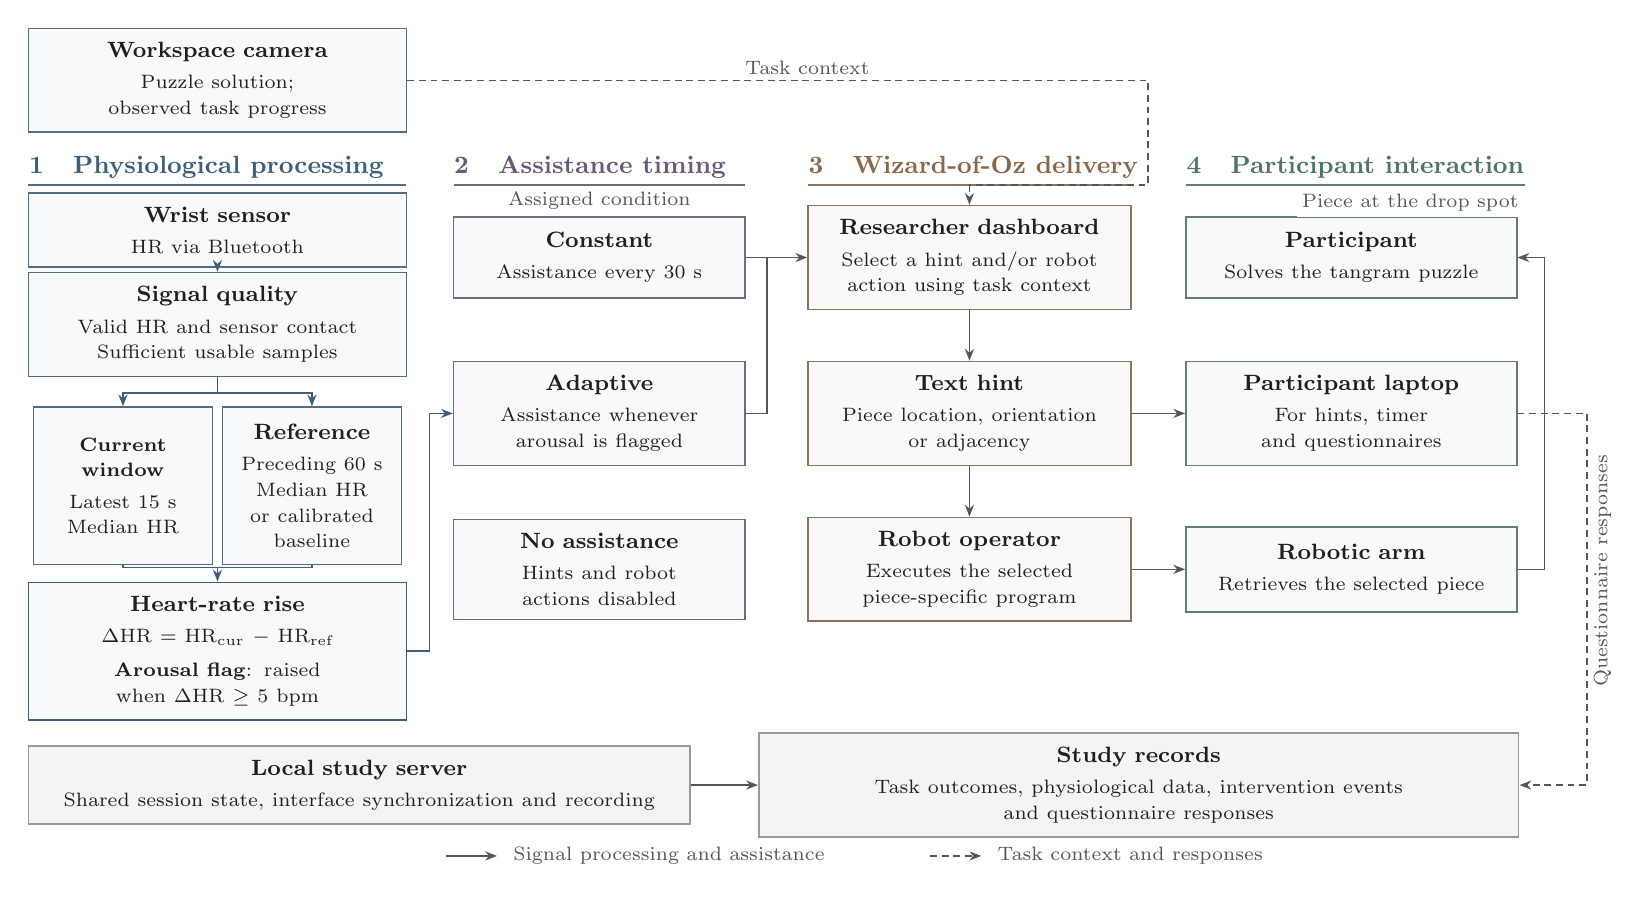
\begin{tikzpicture}[
  font=\rmfamily,text=ink,
  box/.style={draw=rulegray,line width=.55pt,fill=white,align=center,
    inner xsep=5pt,inner ysep=5pt,font=\fontsize{8}{9.3}\selectfont},
  physiological/.style={draw=signal!75!rulegray,fill=signal!4!white},
  timingbox/.style={draw=timing!75!rulegray,fill=timing!4!white},
  deliverybox/.style={draw=delivery!75!rulegray,fill=delivery!4!white},
  participantbox/.style={draw=participant!75!rulegray,fill=participant!4!white},
  head/.style={font=\bfseries\fontsize{9}{10.5}\selectfont,align=left,anchor=west,inner sep=0pt},
  note/.style={font=\fontsize{7.5}{9}\selectfont,text=muted,inner sep=2pt,fill=white},
  arrow/.style={-{Stealth[length=1.5mm,width=1.15mm]},draw=muted,line width=.55pt},
  sig/.style={arrow,draw=signal},
  context/.style={arrow,dashed,dash pattern=on 2.5pt off 1.7pt},
  line/.style={draw=muted,line width=.55pt}
]
\hyphenpenalty=10000
\exhyphenpenalty=10000
% Four headings, without enclosing panels or decorative icons.
\node[head,text=signal] at (0,6.65) {1\quad Physiological processing};
\node[head,text=timing] at (5.4,6.65) {2\quad Assistance timing};
\node[head,text=delivery] at (9.9,6.65) {3\quad Wizard-of-Oz delivery};
\node[head,text=participant] at (14.7,6.65) {4\quad Participant interaction};
\foreach \left/\right/\accent in {0/4.8/signal,5.4/9.1/timing,9.9/14.0/delivery,14.7/19.0/participant}
  \draw[draw=\accent!75!rulegray,line width=.5pt] (\left,6.42)--(\right,6.42);

% Task context is independent of the physiological signal.
\node[box,physiological,text width=4.45cm] (camera) at (2.4,7.75)
  {\textbf{Workspace camera}\\[2pt]
   \labeltext{Puzzle solution; observed task progress}};

% Physiological processing. The parallel windows feed one detector.
\node[box,physiological,text width=4.45cm] (sensor) at (2.4,5.85)
  {\textbf{Wrist sensor}\\[2pt]\labeltext{HR via Bluetooth}};
\node[box,physiological,text width=4.45cm] (quality) at (2.4,4.65)
  {\textbf{Signal quality}\\[2pt]\labeltext{Valid HR and sensor contact}\\
   \labeltext{Sufficient usable samples}};
\node[box,physiological,text width=1.92cm,minimum height=2.00cm] (current) at (1.2,2.60)
  {{\fontsize{7}{8.3}\selectfont\textbf{Current window}}\\[2pt]\labeltext{Latest 15 s}\\\labeltext{Median HR}};
\node[box,physiological,text width=1.92cm,minimum height=2.00cm] (reference) at (3.6,2.60)
  {\textbf{Reference}\\[2pt]\labeltext{Preceding 60 s}\\\labeltext{Median HR}\\
   \labeltext{or calibrated baseline}};
\node[box,physiological,text width=4.45cm,minimum height=1.20cm,draw=signal] (detector) at (2.4,.50)
  {\textbf{Heart-rate rise}\\[2pt]
   \labeltext{$\Delta$HR $=$ HR\textsubscript{cur} $-$ HR\textsubscript{ref}}\\[3pt]
   \labeltext{\textbf{Arousal flag}: raised when $\Delta$HR $\geq$ 5 bpm}};
\draw[sig] (sensor.south)--(quality.north);
\coordinate (split) at ($(quality.south)+(0,-.20)$);
\draw[draw=signal,line width=.55pt] (quality.south)--(split);
\draw[sig] (split)-|(current.north);
\draw[sig] (split)-|(reference.north);
\coordinate (join) at ($(detector.north)+(0,.18)$);
\draw[draw=signal,line width=.55pt] (current.south)|-(join);
\draw[draw=signal,line width=.55pt] (reference.south)|-(join);
\draw[sig] (join)--(detector.north);

% Three assigned conditions are alternatives, not sequential stages.
\node[note,anchor=south] at (7.25,6.04) {Assigned condition};
\node[box,timingbox,text width=3.35cm,minimum height=1.03cm] (constant) at (7.25,5.50)
  {\textbf{Constant}\\[2pt]\labeltext{Assistance every 30 s}};
\node[box,timingbox,text width=3.35cm,minimum height=1.08cm] (adaptive) at (7.25,3.52)
  {\textbf{Adaptive}\\[2pt]\labeltext{Assistance whenever}\\\labeltext{arousal is flagged}};
\node[box,timingbox,text width=3.35cm,minimum height=1.08cm] (none) at (7.25,1.54)
  {\textbf{No assistance}\\[2pt]\labeltext{Hints and robot actions disabled}};
\draw[sig] (detector.east)--++(.28,0)|-(adaptive.west);

% Human-operated delivery and its two outputs.
\node[box,deliverybox,text width=3.75cm,minimum height=1.03cm] (dashboard) at (11.95,5.50)
  {\textbf{Researcher dashboard}\\[2pt]\labeltext{Select a hint and/or robot}\\
   \labeltext{action using task context}};
\node[box,deliverybox,text width=3.75cm,minimum height=1.08cm] (hint) at (11.95,3.52)
  {\textbf{Text hint}\\[2pt]\labeltext{Piece location, orientation}\\\labeltext{or adjacency}};
\node[box,deliverybox,text width=3.75cm,minimum height=1.08cm] (operator) at (11.95,1.54)
  {\textbf{Robot operator}\\[2pt]\labeltext{Executes the selected}\\\labeltext{piece-specific program}};
\coordinate (gate) at ($(dashboard.west)+(-.30,0)$);
\draw[line] (constant.east)--(gate);
\draw[line] (adaptive.east)--++(.27,0)|-(gate);
\draw[arrow] (gate)--(dashboard.west);
\draw[arrow] (dashboard.south)--(hint.north);
\draw[arrow] (hint.south)--(operator.north);

% Participant-facing endpoints remain aligned with delivery.
\node[box,participantbox,text width=3.85cm,minimum height=1.03cm] (person) at (16.8,5.50)
  {\textbf{Participant}\\[2pt]\labeltext{Solves the tangram puzzle}};
\node[box,participantbox,text width=3.85cm,minimum height=1.08cm] (laptop) at (16.8,3.52)
  {\textbf{Participant laptop}\\[2pt]\labeltext{For hints, timer}\\\labeltext{and questionnaires}};
\node[box,participantbox,text width=3.85cm,minimum height=1.08cm] (arm) at (16.8,1.54)
  {\textbf{Robotic arm}\\[2pt]\labeltext{Retrieves the selected piece}};
\draw[arrow] (hint.east)--(laptop.west);
\draw[arrow] (operator.east)--(arm.west);
\coordinate (piece) at ($(arm.east)+(.34,0)$);
\draw[arrow] (arm.east)--(piece)|-(person.east);
\node[note,anchor=east] at (19.00,6.20) {Piece at the drop spot};

% Dashed task-context route stays clear of headings and node labels.
\coordinate (contextRail) at (14.22,7.75);
\coordinate (contextTurn) at ($(dashboard.north)+(0,.25)$);
\draw[line,dashed,dash pattern=on 2.5pt off 1.7pt]
 (camera.east)--node[note,above,pos=.54]{Task context}(contextRail)
 --(contextRail|-contextTurn)--(contextTurn);
\draw[context] (contextTurn)--(dashboard.north);

% Compact footer: shared infrastructure and its recorded outputs.
\node[box,fill=wash,text width=8.05cm,minimum height=.95cm] (server) at (4.2,-1.20)
 {\textbf{Local study server}\\[2pt]
  \labeltext{Shared session state, interface synchronization and recording}};
\node[box,fill=wash,text width=9.30cm,minimum height=.95cm] (records) at (14.10,-1.20)
 {\textbf{Study records}\\[2pt]
  \labeltext{Task outcomes, physiological data, intervention events}\\
  \labeltext{and questionnaire responses}};
\draw[arrow] (server.east)--(records.west);
\coordinate (questionnaire) at ($(laptop.east)+(.88,0)$);
\draw[context] (laptop.east)--(questionnaire)
 --(questionnaire|-records.east)--(records.east);
\node[note,rotate=90] at ($(questionnaire)+(0.20,-2.0)$) {Questionnaire responses};

% Line semantics, kept separate from the diagram's information hierarchy.
\draw[arrow] (5.30,-2.10)--(5.95,-2.10);
\node[note,anchor=west] at (6.08,-2.10) {Signal processing and assistance};
\draw[context] (11.45,-2.10)--(12.10,-2.10);
\node[note,anchor=west] at (12.23,-2.10) {Task context and responses};
\end{tikzpicture}
\end{document}
